\Askhsh{18302}{4}
\begin{ylh}{1}
    \item 10.5. Λόγος εμβαδών όμοιων τριγώνων - πολυγώνων.
\end{ylh}
\begin{wrapfigure}[9]{r}{5cm} % Adjusted line count for wrapfigure
    \centering
    \begin{tikzpicture}[scale=0.8]
        % Define point A as the origin
        \tkzDefPoint(0,0){A}
        
        % Define points B, D on a line passing through A (horizontal line)
        % A is between B and D.
        % For visual consistency with the problem (e.g., AD=2AB):
        \tkzDefPoint(-2.5,0){B} % Let AB be 2.5 units
        \tkzDefPoint(5,0){D}    % Let AD be 5 units (so AD=2AB)
        
        % Define points G, E on a line passing through A (slanted line)
        % A is between G and E.
        % For visual consistency with the problem (e.g., AE=0.5AG):
        % Let G be in the upper-left quadrant from A, as in the original image.
        \tkzDefPoint(-1.5,3.5){G} % Coordinates for Gamma (upper-left from A)
        % Calculate E based on A, G and AE = 0.5 AG
        % Vector AG = (-1.5, 3.5). Vector AE = -0.5 * AG = (0.75, -1.75).
        \tkzDefPoint(0.75,-1.75){E} % Coordinates for E (lower-right from A, collinear with G,A)
        
        % Draw all visible segments as in the original image
        \tkzDrawSegment[thick](B,G)
        \tkzDrawSegment[thick](G,A)
        \tkzDrawSegment[thick](A,B)
        \tkzDrawSegment[thick](A,D)
        \tkzDrawSegment[thick](A,E)
        \tkzDrawSegment[thick](D,E)
        
        % Draw the points
        \tkzDrawPoints(A,B,G,D,E)
        
        % Label the points
        \tkzLabelPoint[below right](A){A}
        \tkzLabelPoint[below left](B){B}
        \tkzLabelPoint[above left](G){$\Gamma$}
        \tkzLabelPoint[below right](D){$\Delta$}
        \tkzLabelPoint[below](E){E} % Positioned below E for clarity
    \end{tikzpicture}
\end{wrapfigure}
Σε τρίγωνο \mbox{AB$\Gamma$} προεκτείνουμε τις πλευρές \mbox{BA} και \mbox{$\Gamma$A} κατά τμήματα \mbox{A$\Delta$} και \mbox{AE} αντίστοιχα, όπως φαίνεται στο σχήμα.

\begin{alist}
    \item Αν είναι \mbox{A$\Delta = 2$AB} και \mbox{AE = $\dfrac{1}{2}$A$\Gamma$}, να αποδείξετε ότι τα τρίγωνα \mbox{A$\Delta$E} και \mbox{AB$\Gamma$} είναι ισοδύναμα. \monades{09}
    \item Αν προεκτείνουμε τις πλευρές \mbox{BA} και \mbox{$\Gamma$A} κατά τμήματα είναι \mbox{A$\Delta = \mu \cdot$ AB} και \mbox{AE = $\nu \cdot$ A$\Gamma$} αντίστοιχα, όπου \mbox{$\mu, \nu$} είναι θετικοί πραγματικοί αριθμοί, ποια πρέπει να είναι η σχέση των αριθμών \mbox{$\mu$} και \mbox{$\nu$} ώστε τα τρίγωνα \mbox{A$\Delta$E} και \mbox{AB$\Gamma$} να είναι ισοδύναμα; \monades{10}
    \item Αν είναι \mbox{A$\Gamma = \dfrac{3}{2}$AB} και \mbox{A$\Delta = 2$AB}, να βρείτε τις δυνατές θέσεις του \mbox{E} ώστε τα \mbox{AB$\Gamma$} και \mbox{A$\Delta$E} να είναι όμοια. \monades{06}
\end{alist}